\chapter{Usage}
\label{chap:usage}

In the previous chapters, we have delved into the design decisions behind DortDB, its implementation, and its theoretical background. However, we have not yet described how to actually use it or extend it. This chapter will serve as a walkthrough through user interaction and as a concise manual for developers. It does not aim to be a full-fledged documentation of DortDB.

\section{Showcase}

DortDB Showcase is a GUI intended as a demonstration of DortDB's capabilities. While it is possible to run the demo locally, the recommended way is to use an instance deployed to GitHub Pages at \url{https://filipjezek.github.io/dortdb}. The Showcase is a purely frontend single page application written in Angular. The user can write queries and inspect their logical plans, experimenting with various optimizer rules. It is also possible to execute the queries on the UniBench sample dataset used in benchmarks in section \ref{sec:unibench}. The rest of this section will consist of a sequence of figures describing various parts of the user interface.

\begin{figure}[!h]
    \centering
    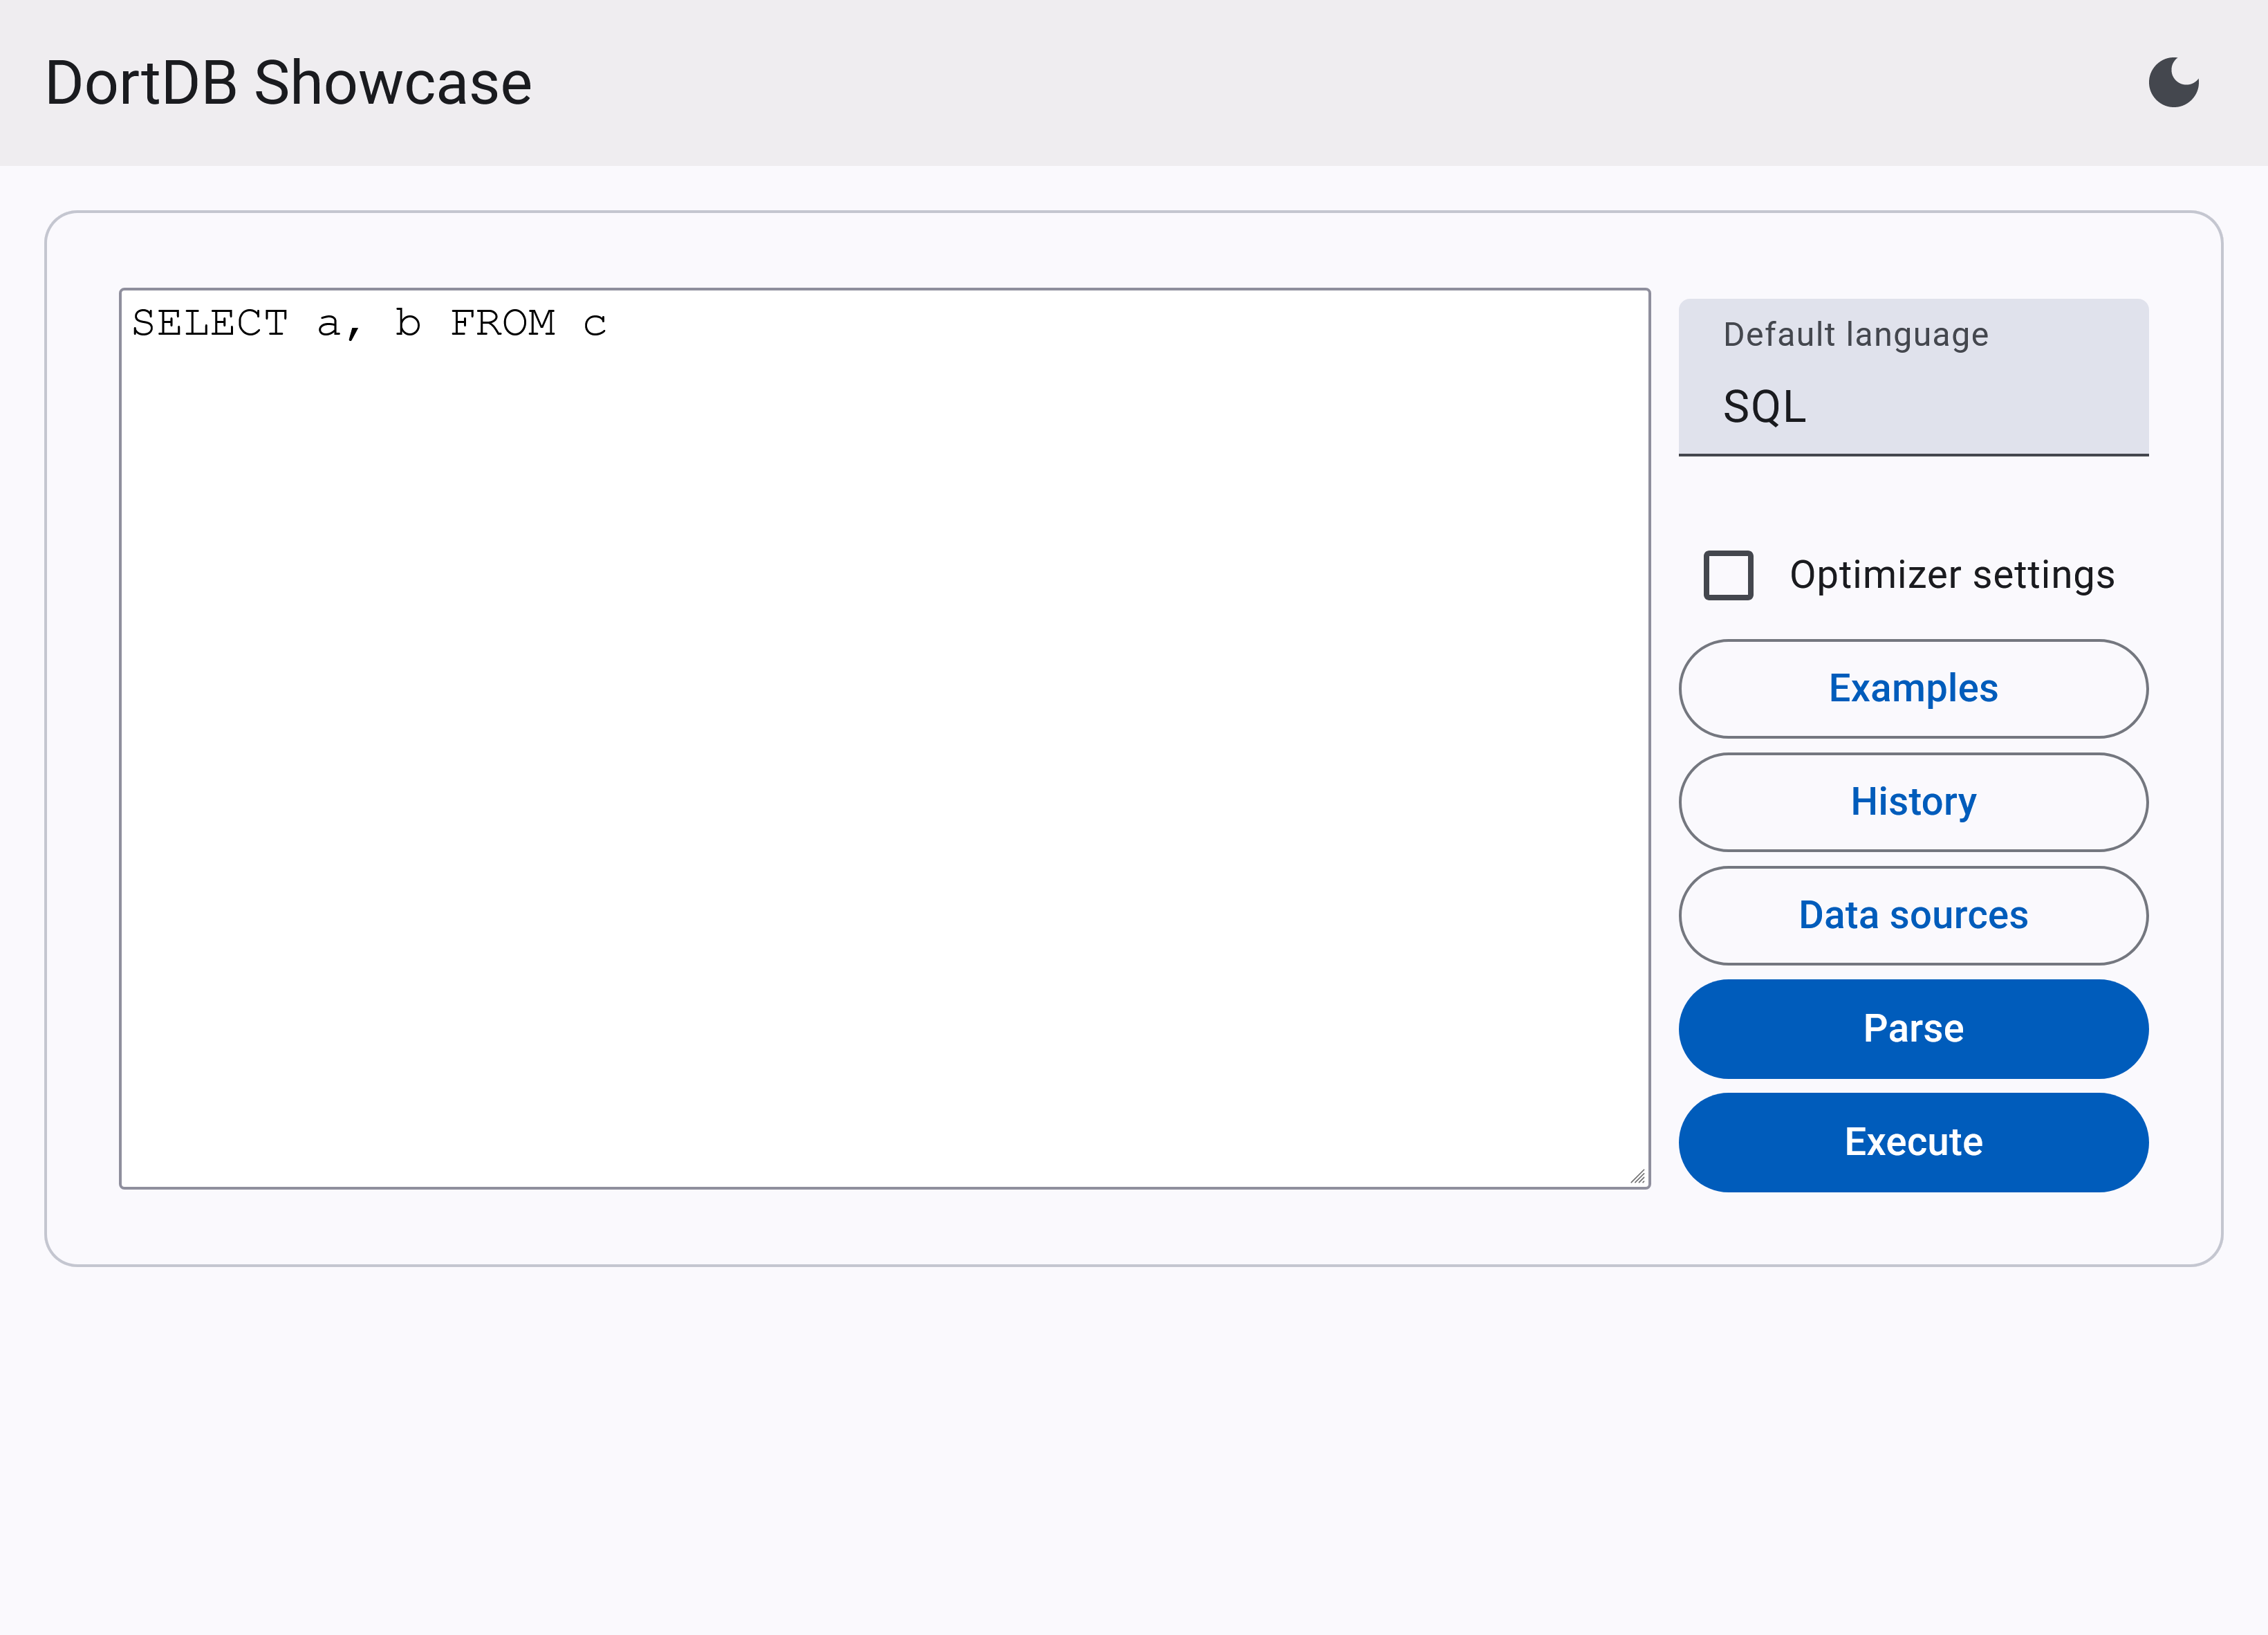
\includegraphics[width=0.8\linewidth]{img/showcase_initial.png}
    \caption{Showcase when loaded in the web browser. The application remembers all settings, including the current query, the optimizer settings, the default language, and query history.}
\end{figure}

\begin{figure}[!h]
    \centering
    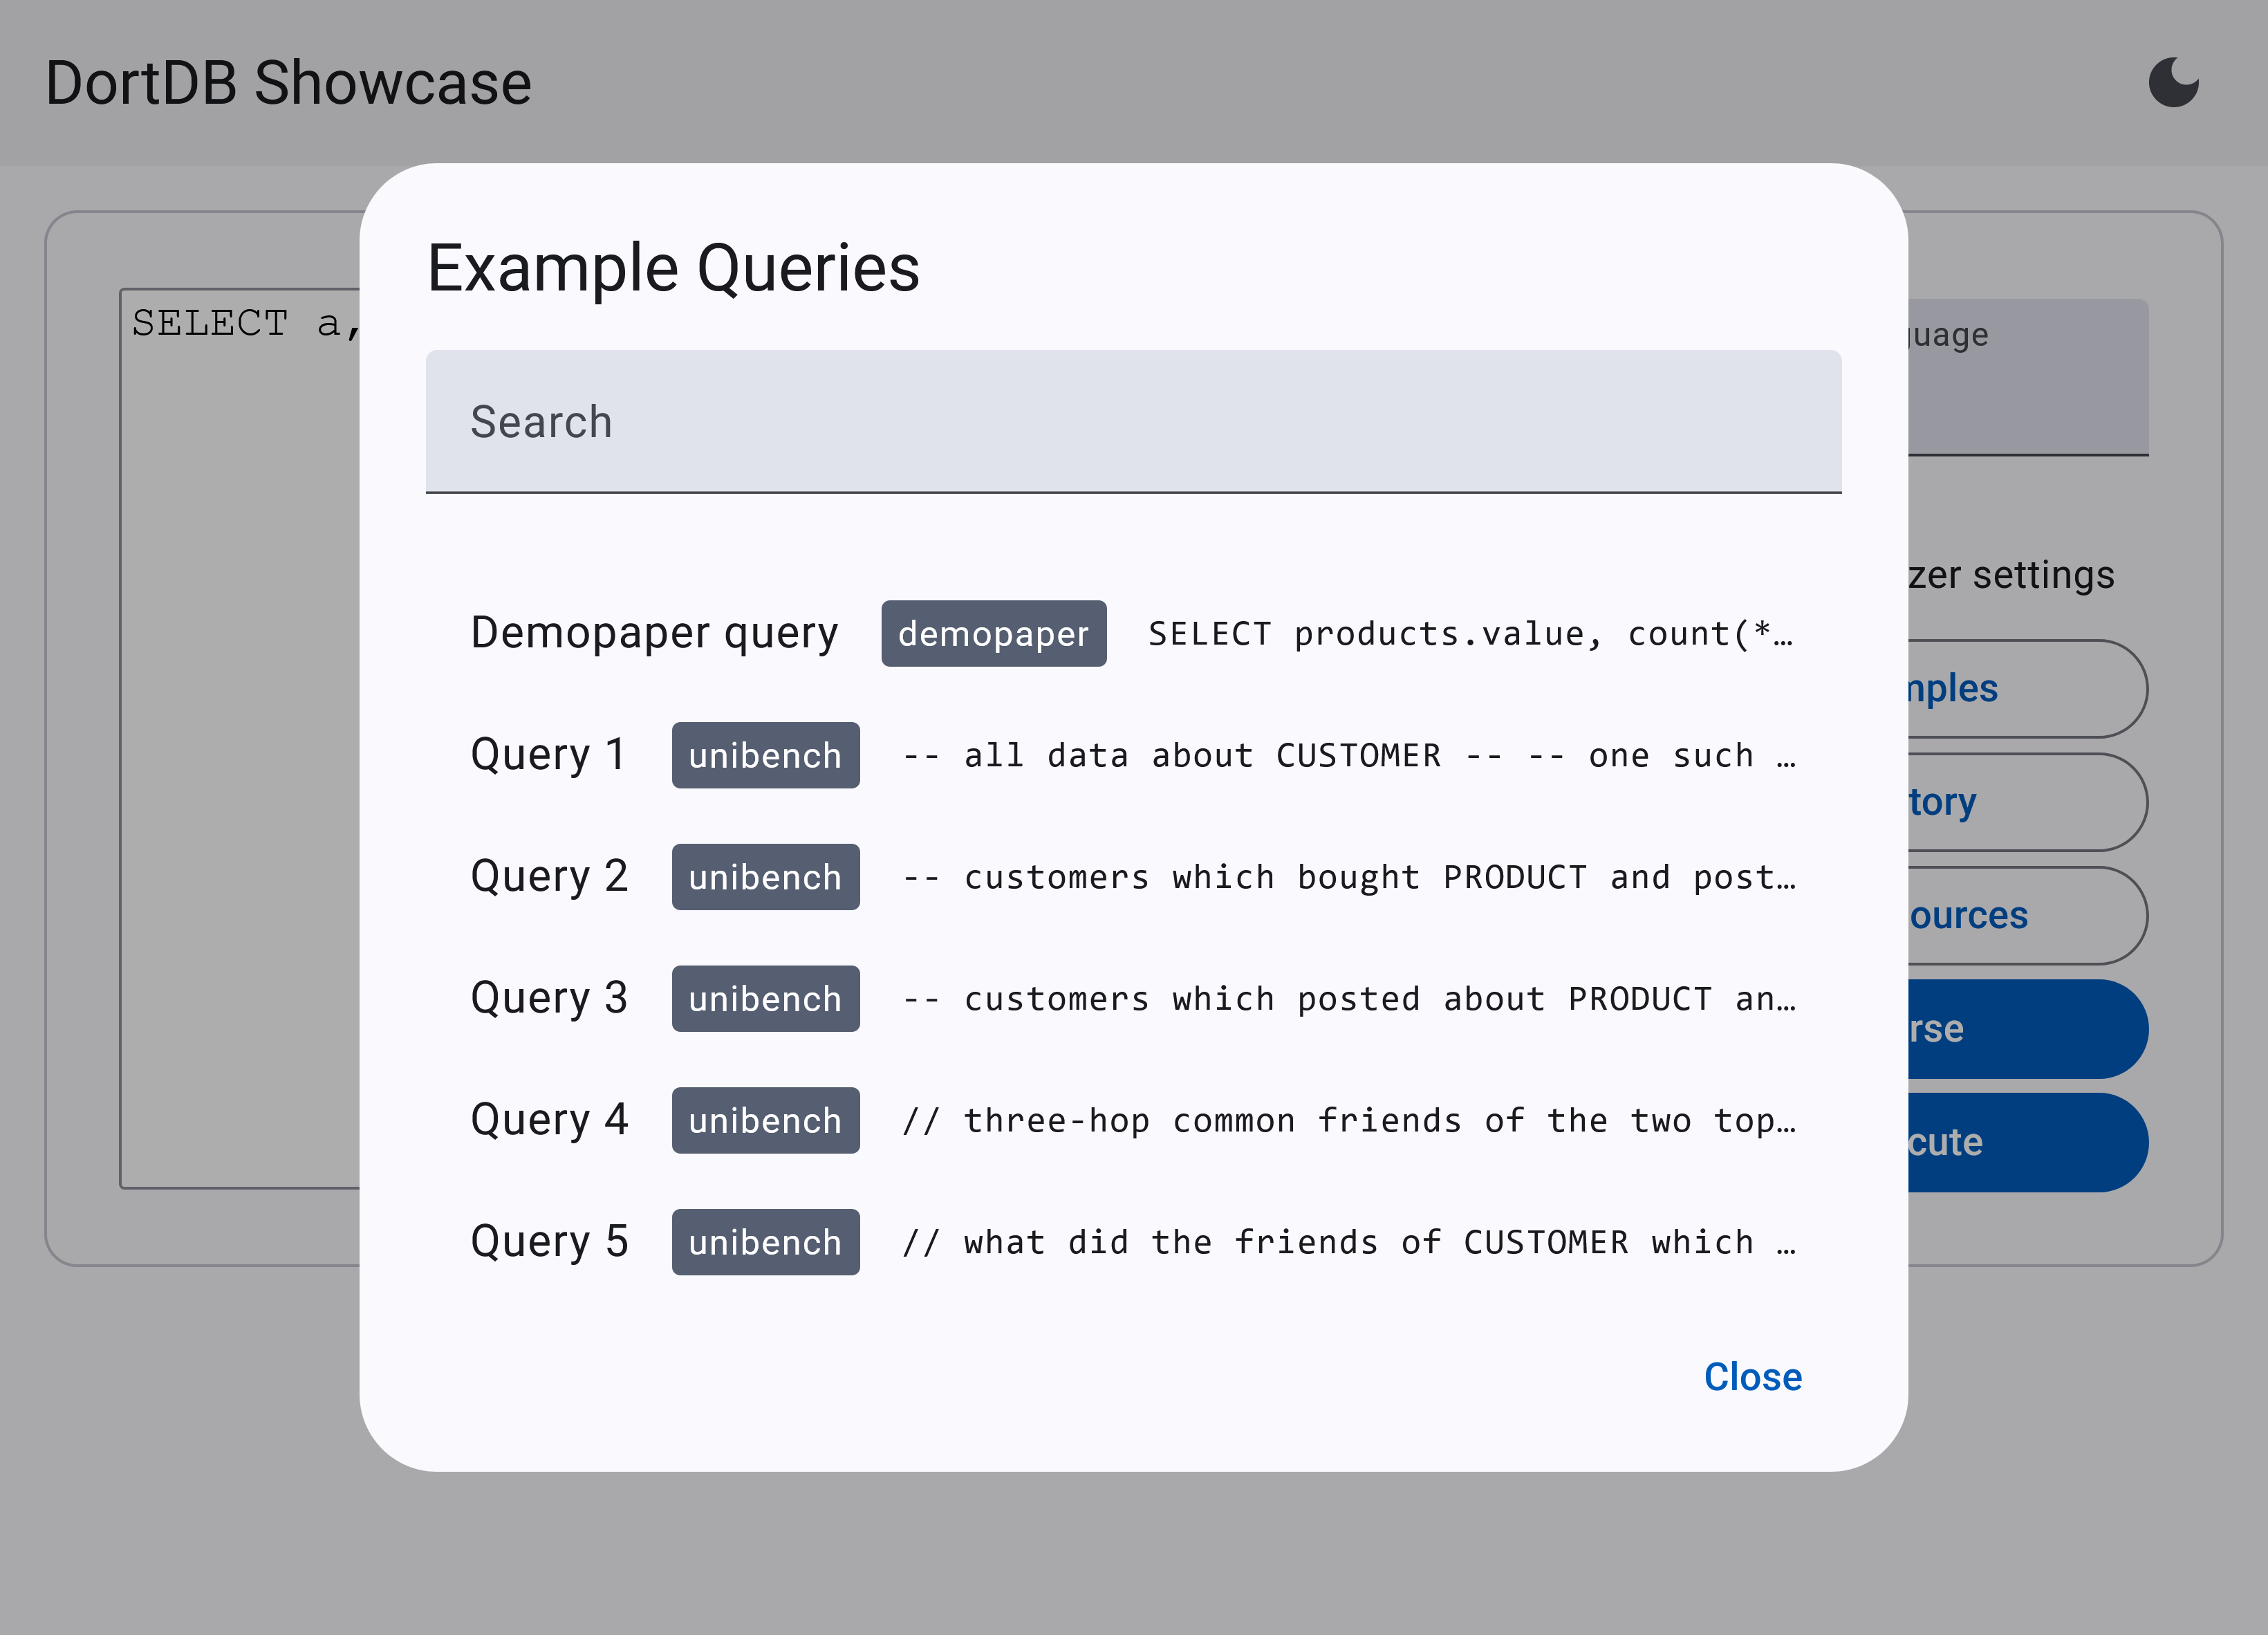
\includegraphics[width=0.8\linewidth]{img/showcase_example_queries.png}
    \caption{Showcase example queries. In order to help the user properly try out DortDB, this dialog offers a quick way to find interesting examples.}
\end{figure}

\begin{figure}[!h]
    \centering
    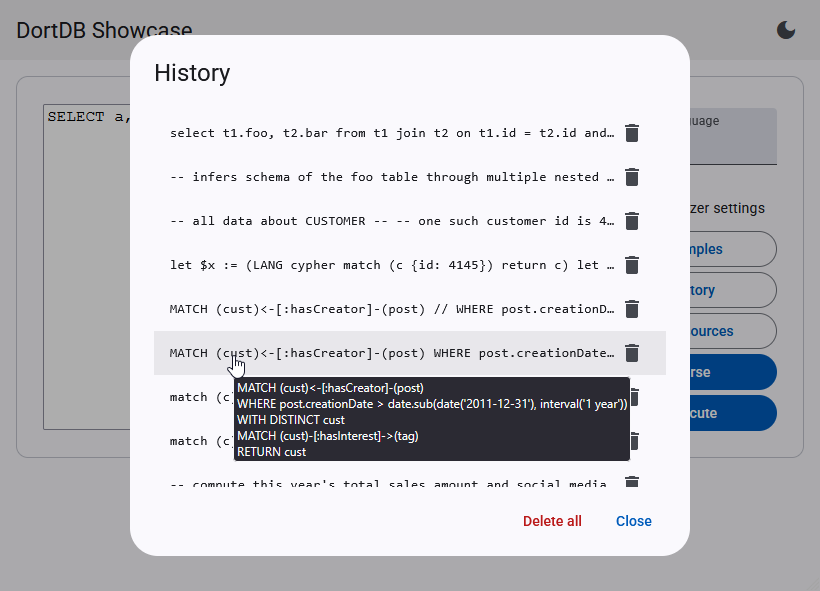
\includegraphics[width=0.8\linewidth]{img/showcase_history.png}
    \caption{Showcase query history. The history remembers the last 20 parsed or executed queries.}
\end{figure}

\begin{figure}[!h]
    \centering
    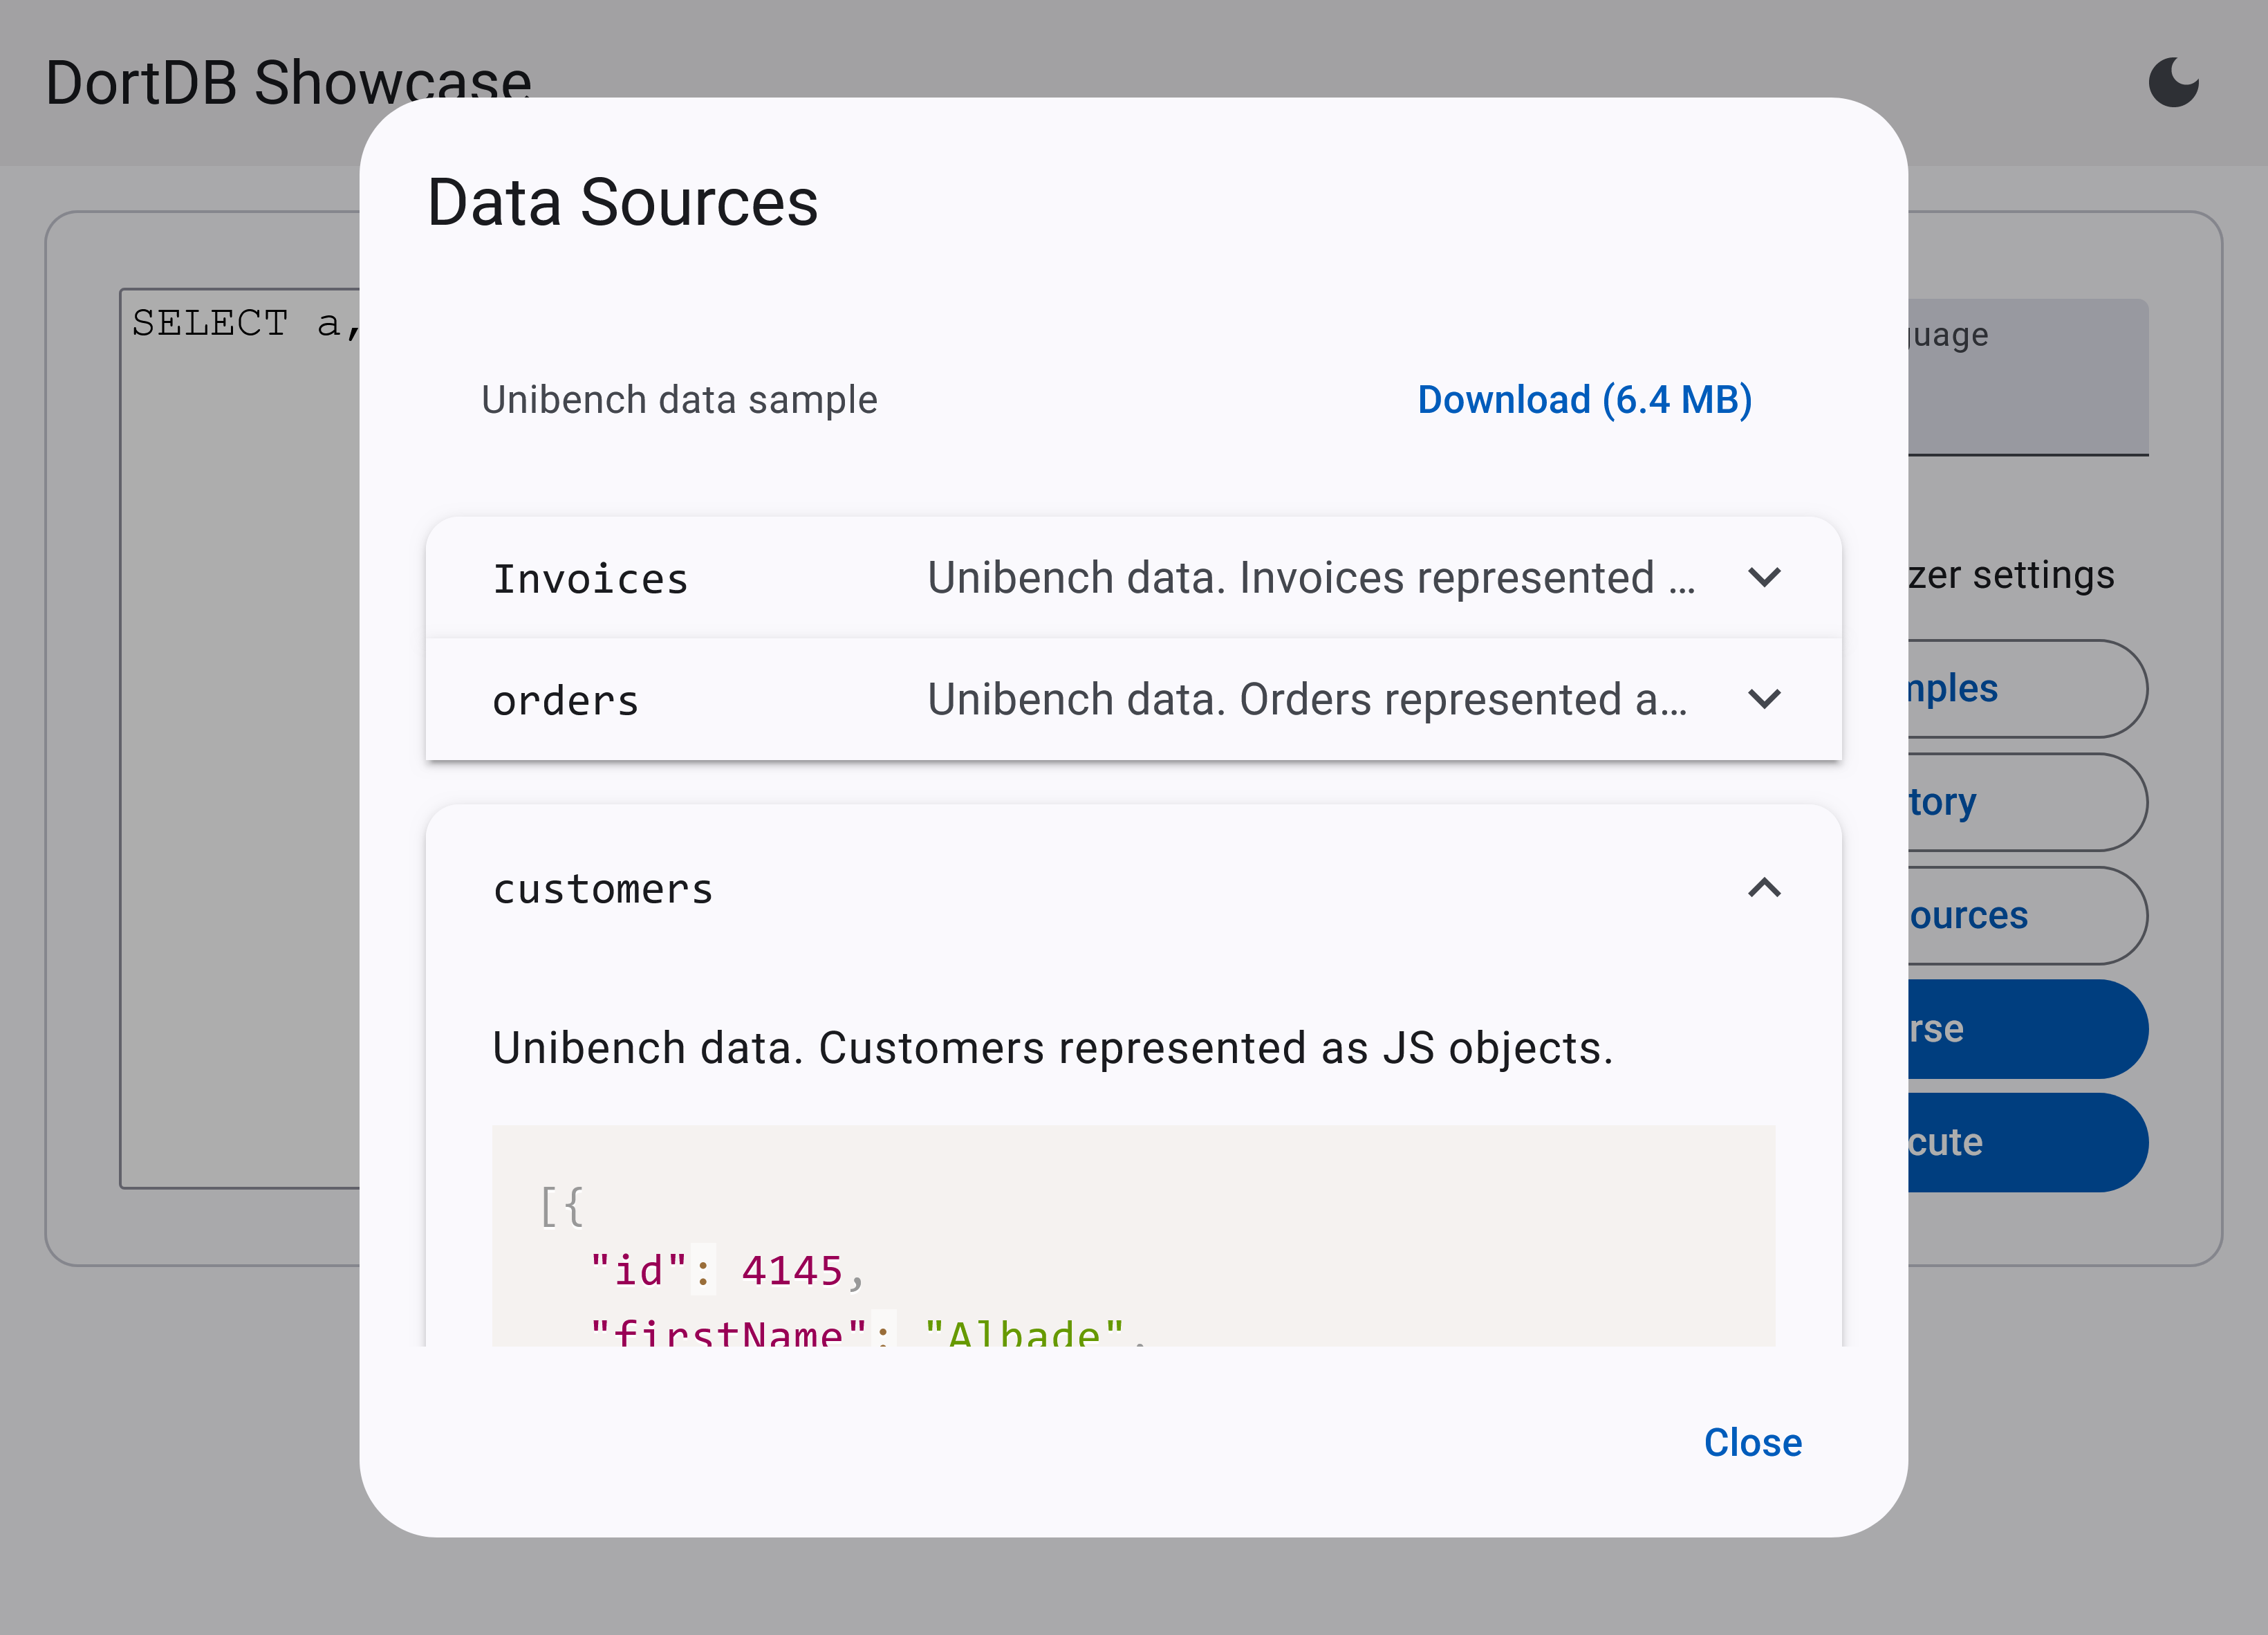
\includegraphics[width=0.8\linewidth]{img/showcase_data_sources.png}
    \caption{Showcase data sources. Showcase allows users to download a sample of the UniBench data and register it as data sources. The individual data sources are described in collapsible expansion panels. Once the user downloads the data, the dialog offers to save the parsed data into the web browser to avoid redownloading it when the page is refreshed.}
\end{figure}

\begin{figure}[!h]
    \centering
    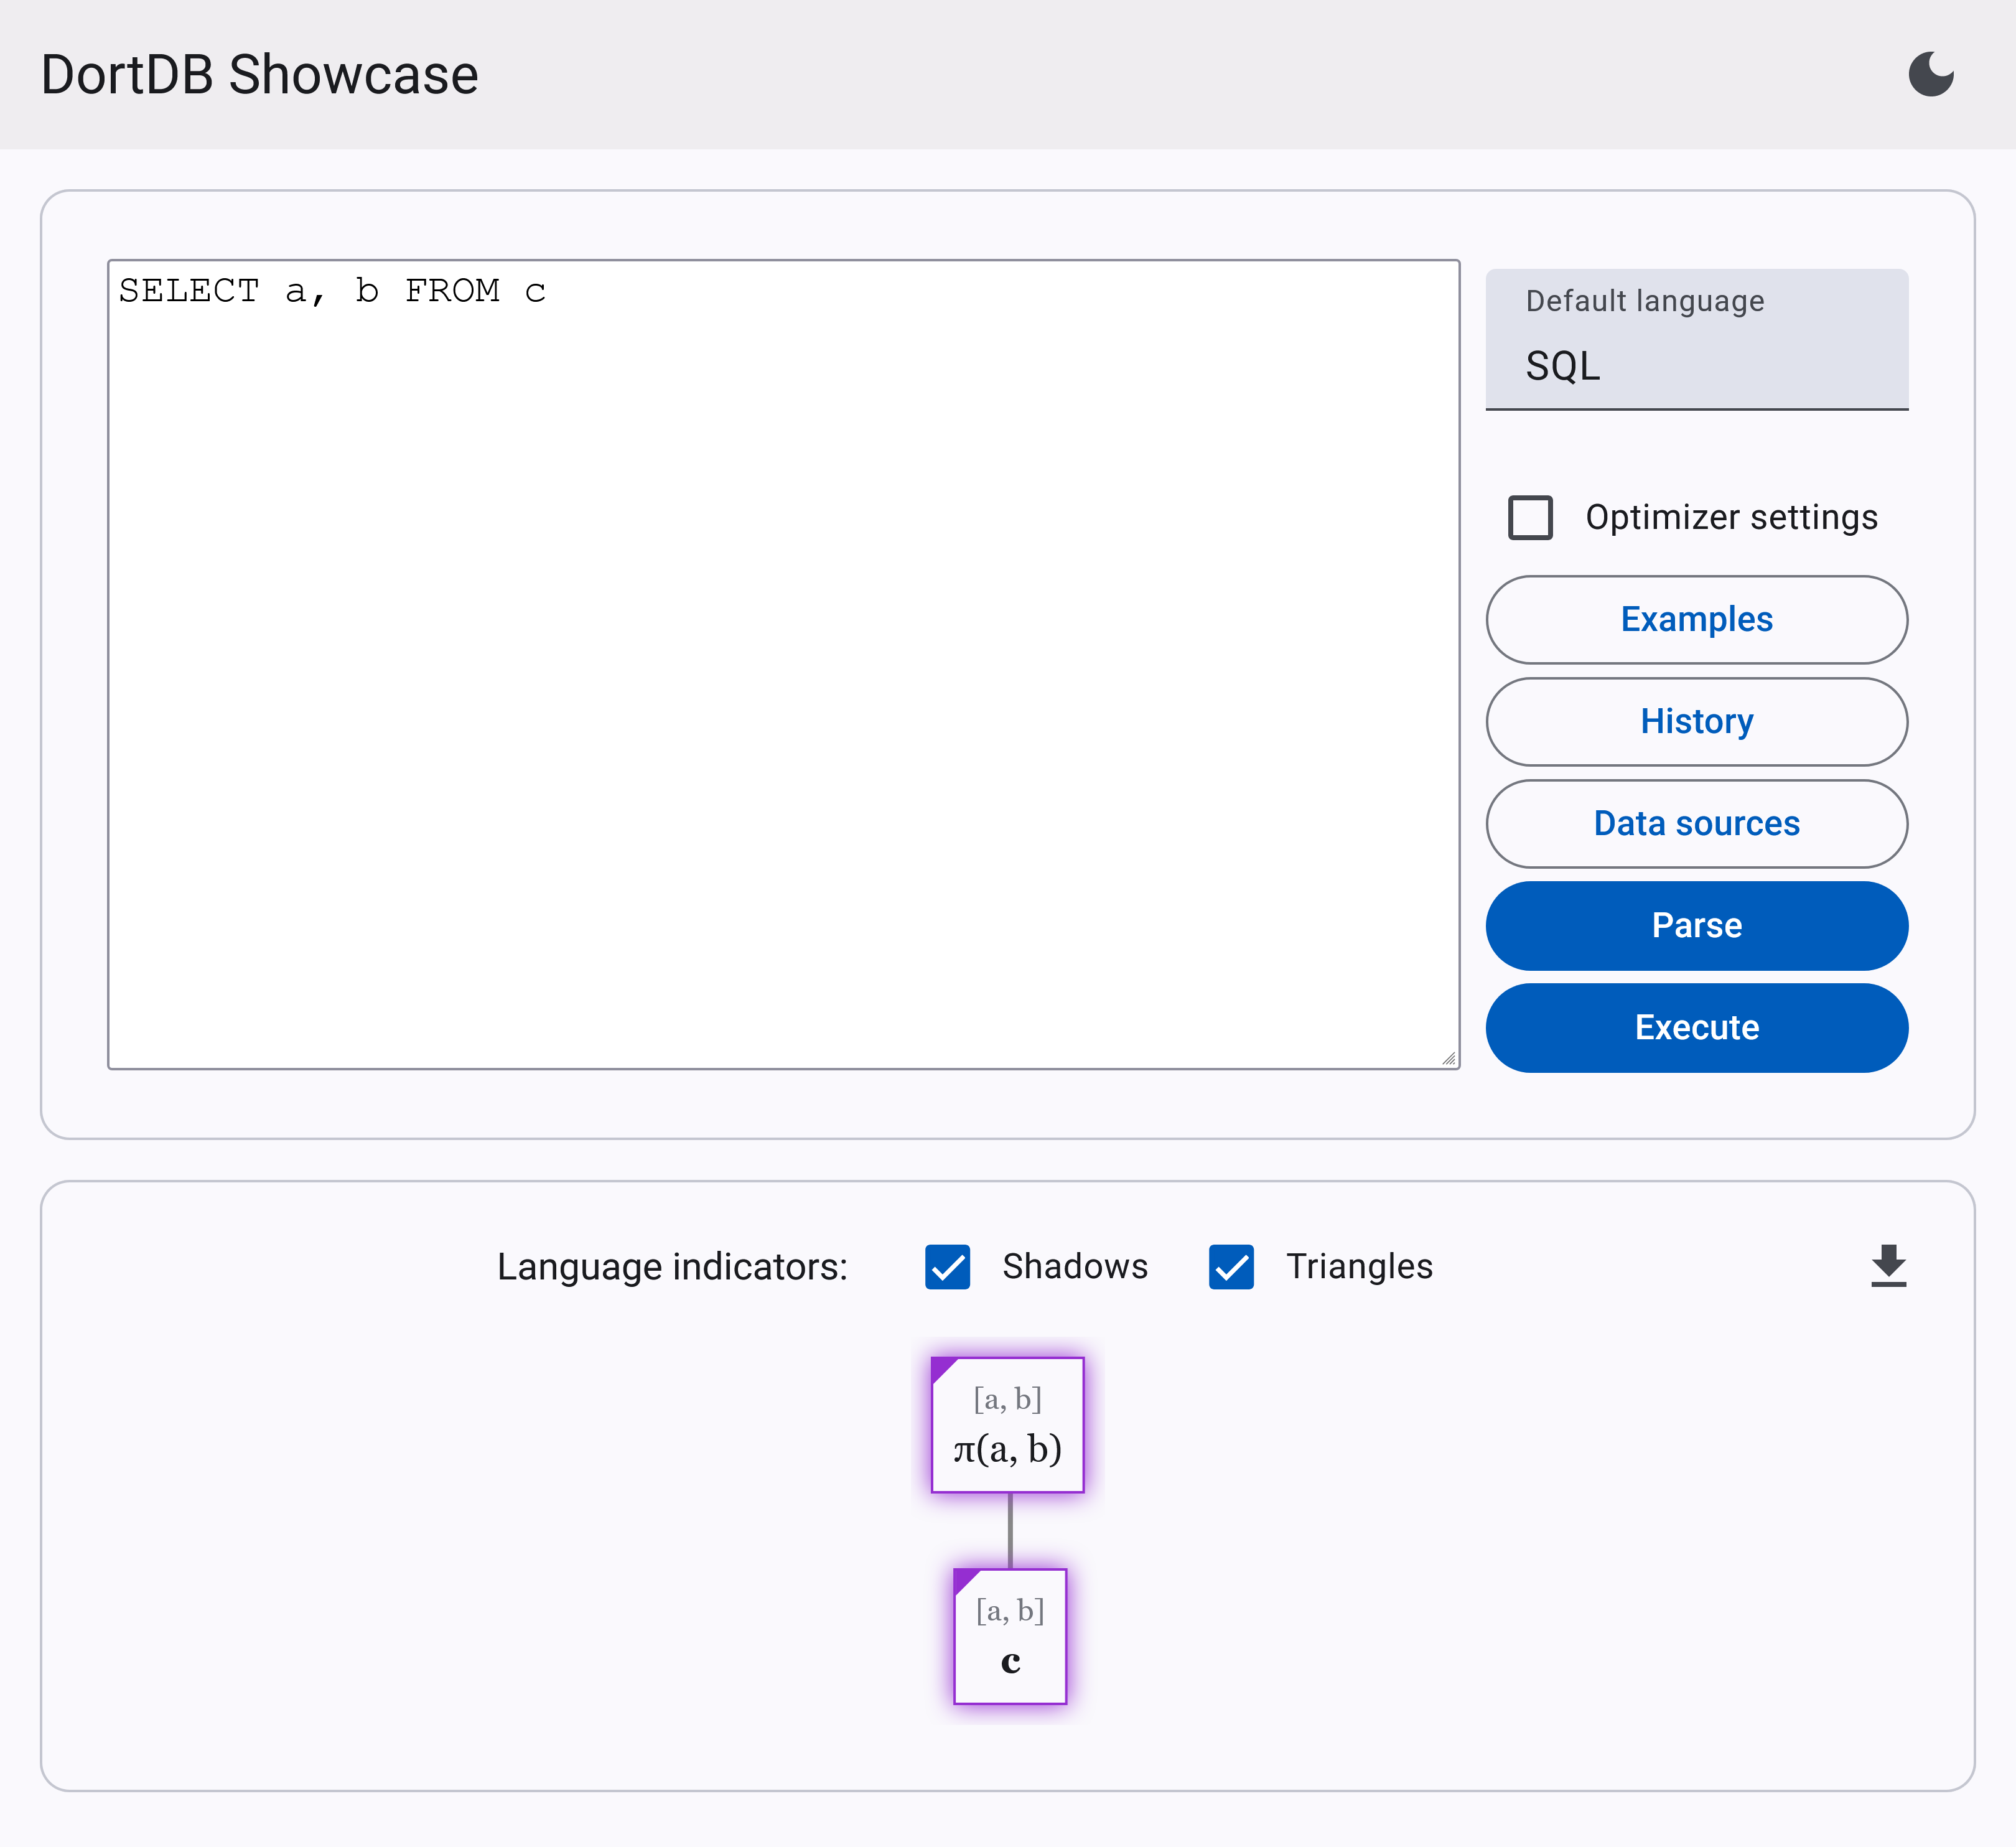
\includegraphics[width=0.8\linewidth]{img/showcase_parse.png}
    \caption{When the query is parsed, the logical plan is displayed as an interactive tree, similar to previous figures in this thesis. The tree can be zoomed and panned. It is possible to download the tree as a PNG image.}
\end{figure}

\begin{figure}[!h]
    \centering
    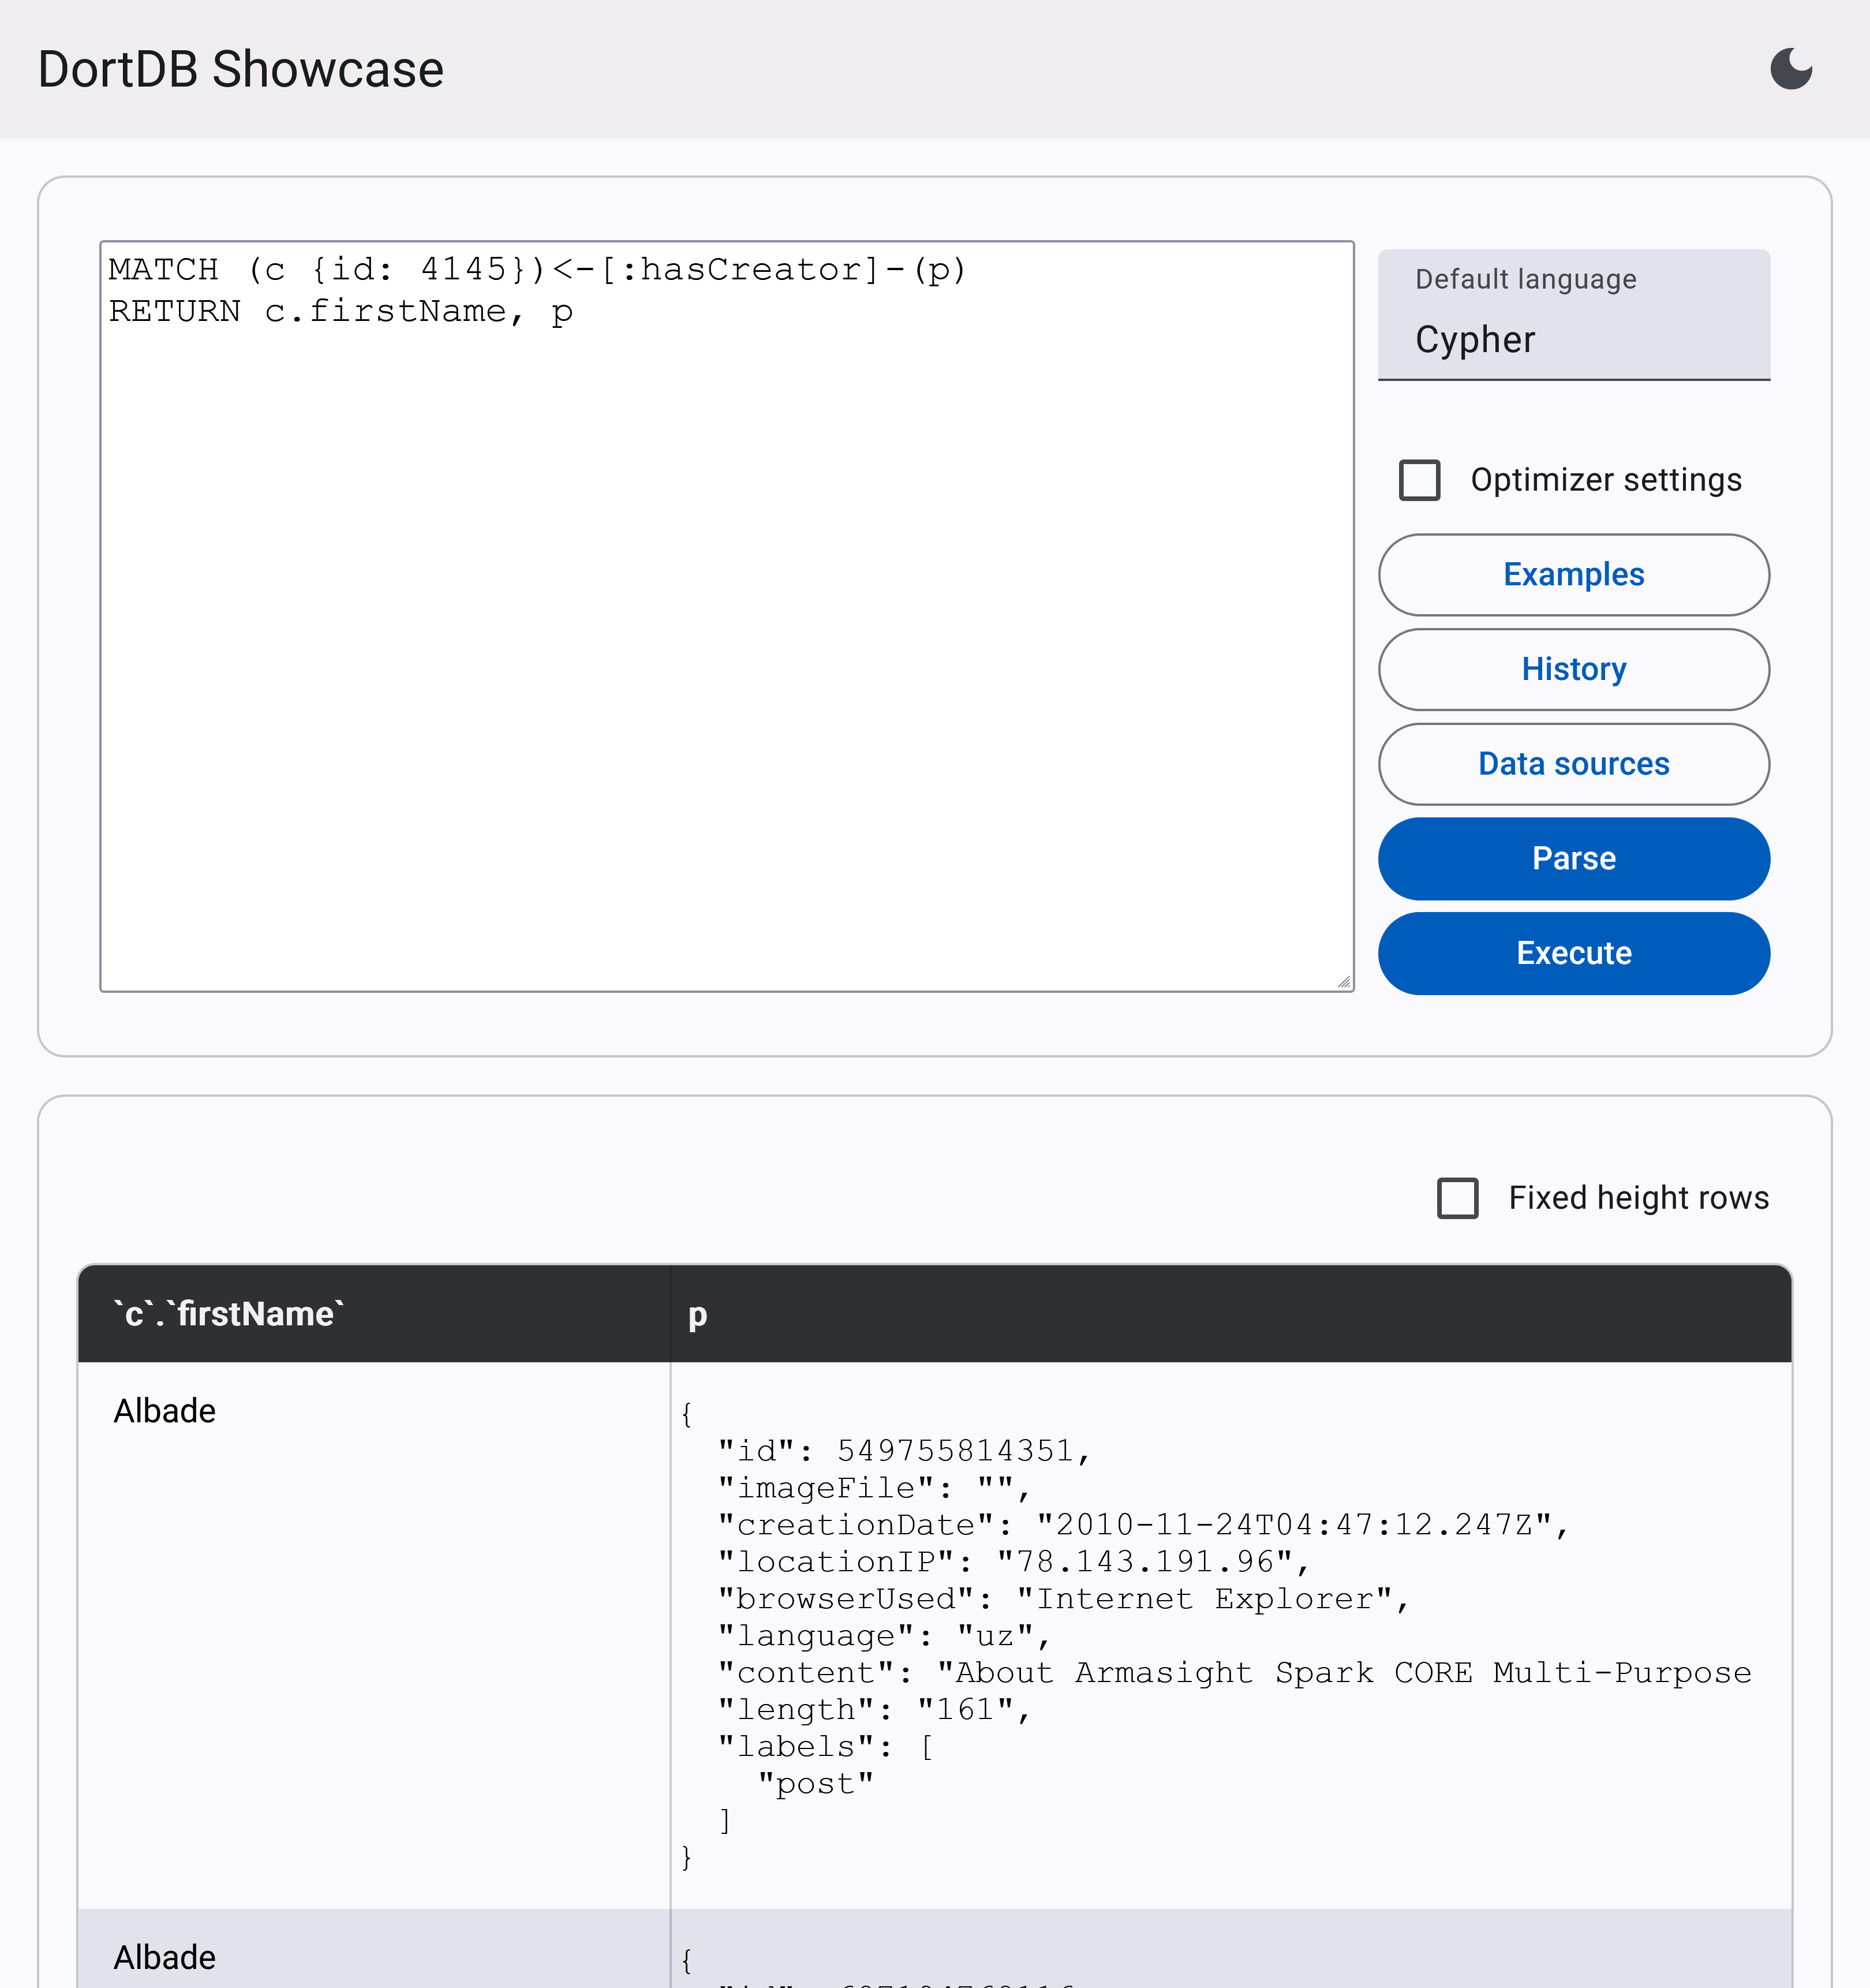
\includegraphics[width=0.8\linewidth]{img/showcase_execute.png}
    \caption{The results of the query execution are displayed in a paginated table. The table columns have adjustable widths.}
\end{figure}

\begin{figure}[!h]
    \centering
    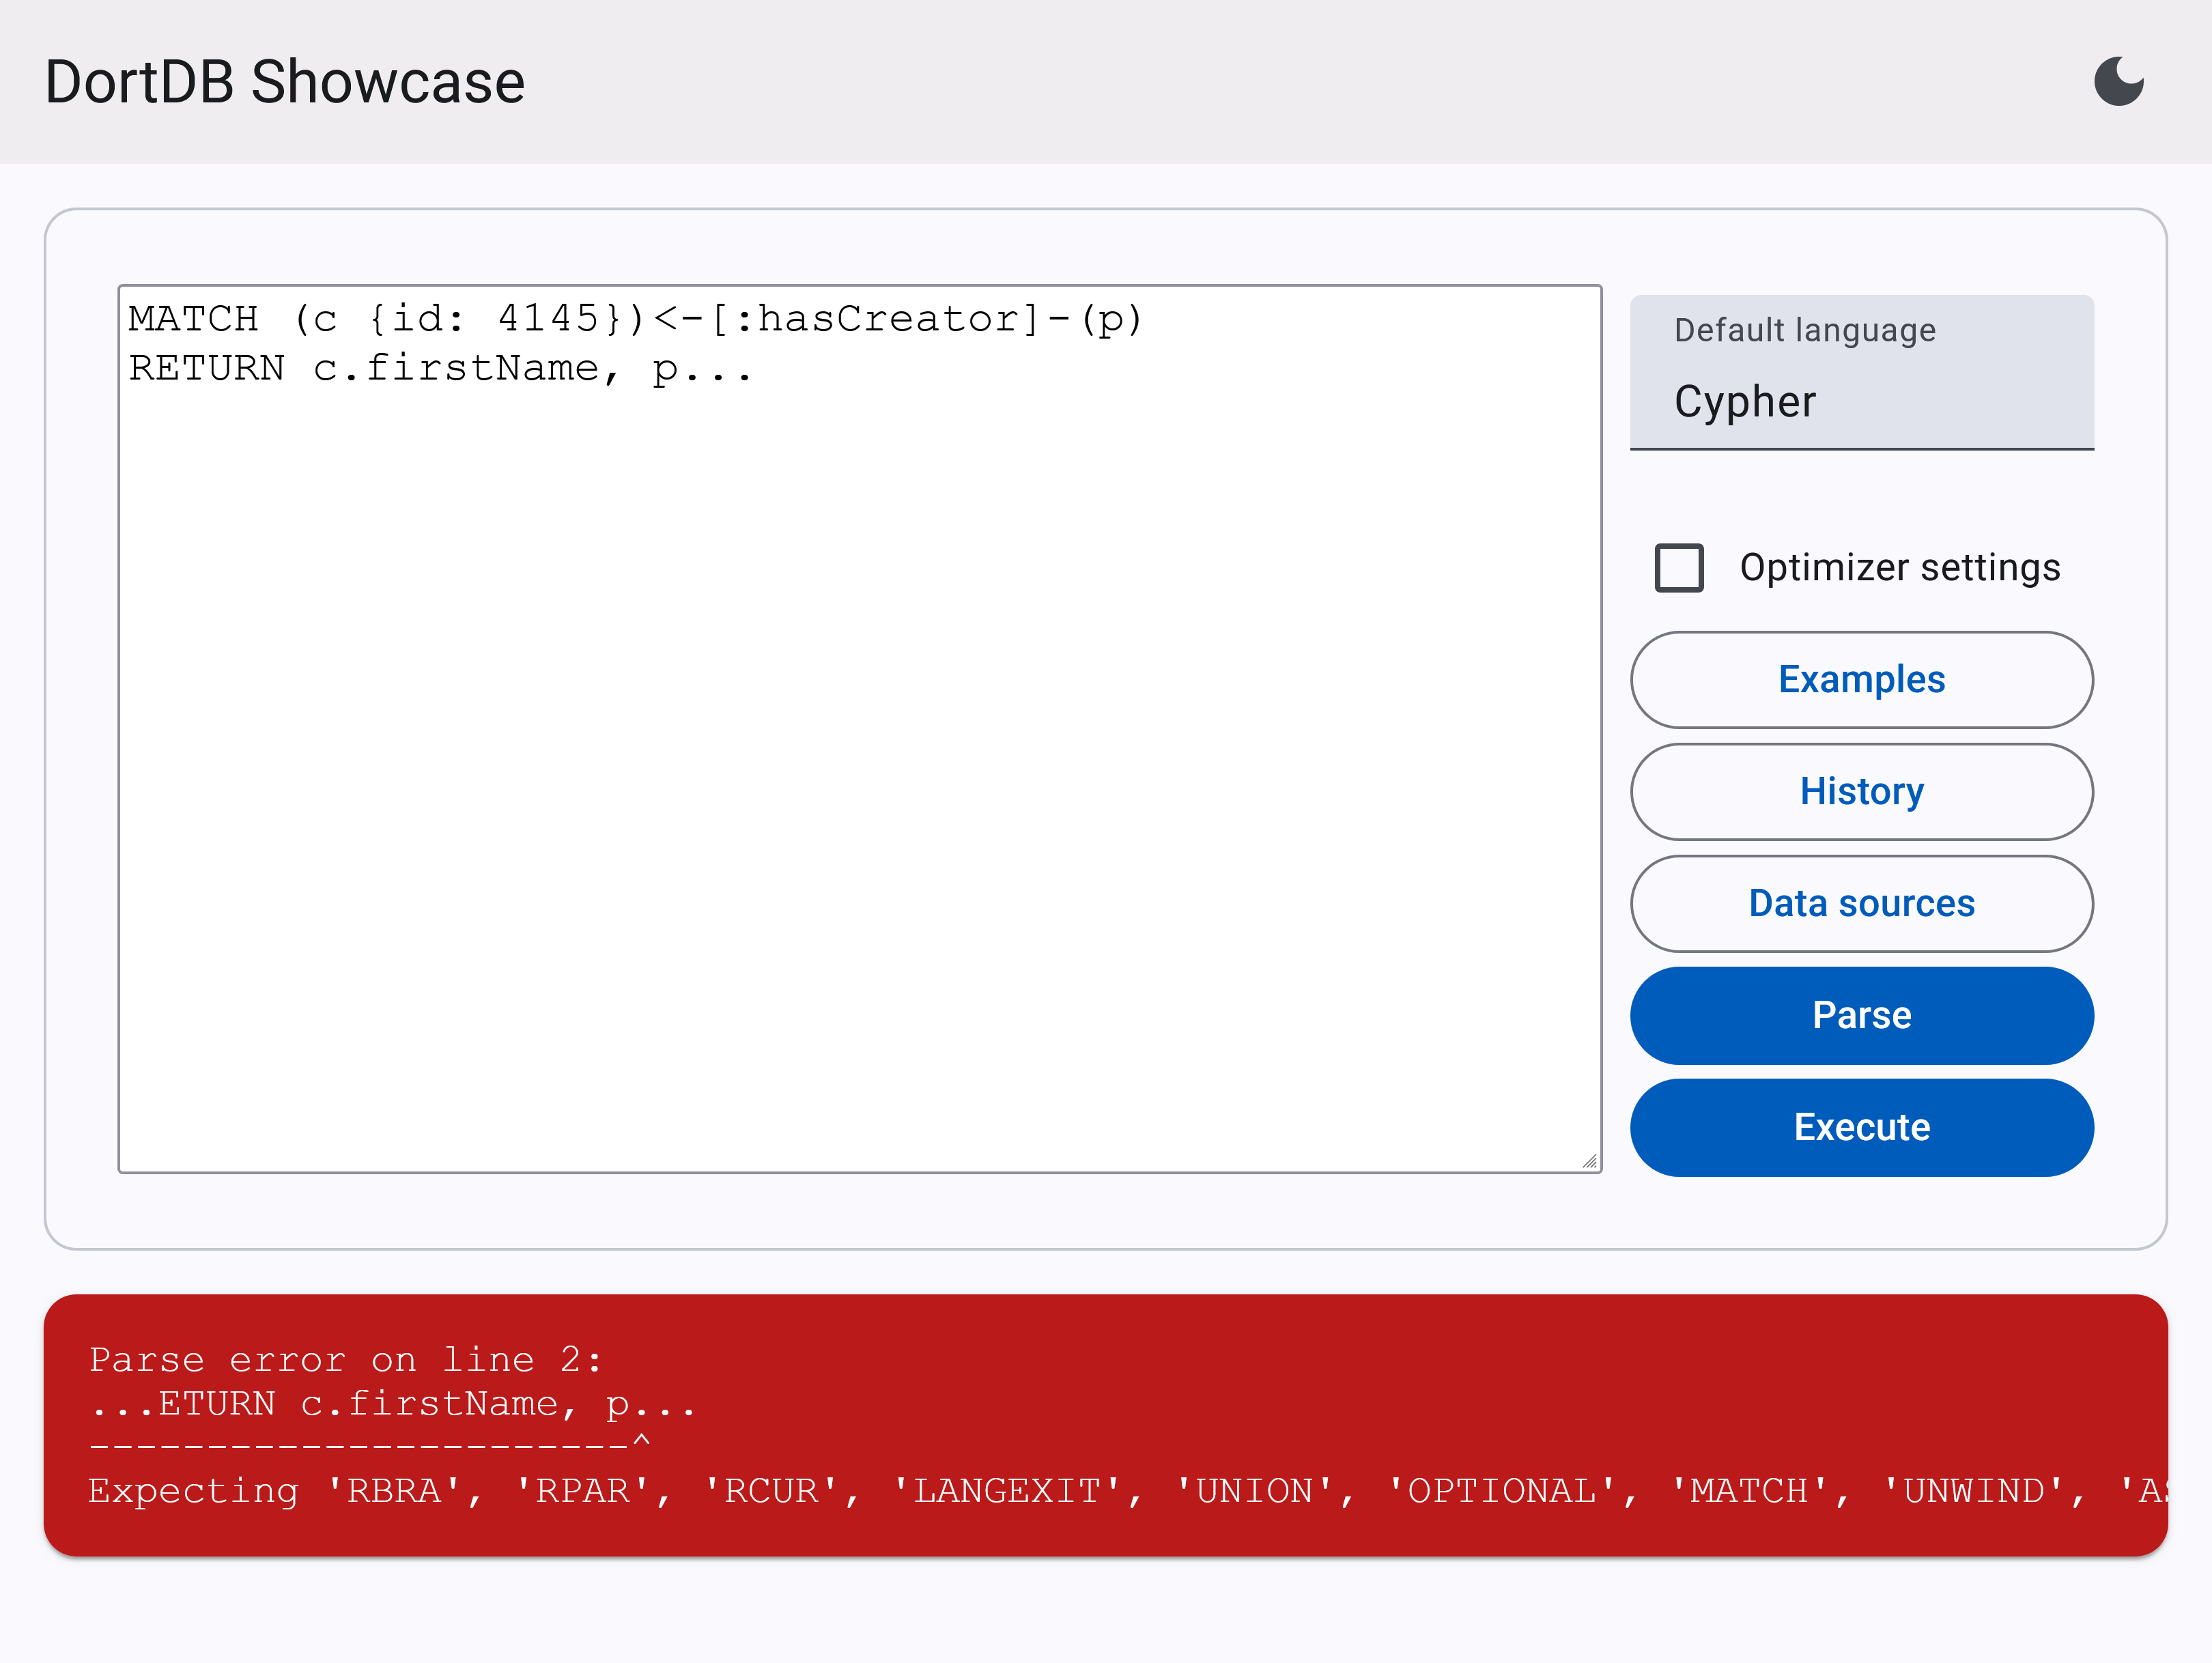
\includegraphics[width=0.8\linewidth]{img/showcase_error.png}
    \caption{Query errors are displayed to the user.}
\end{figure}

\begin{figure}[!h]
    \centering
    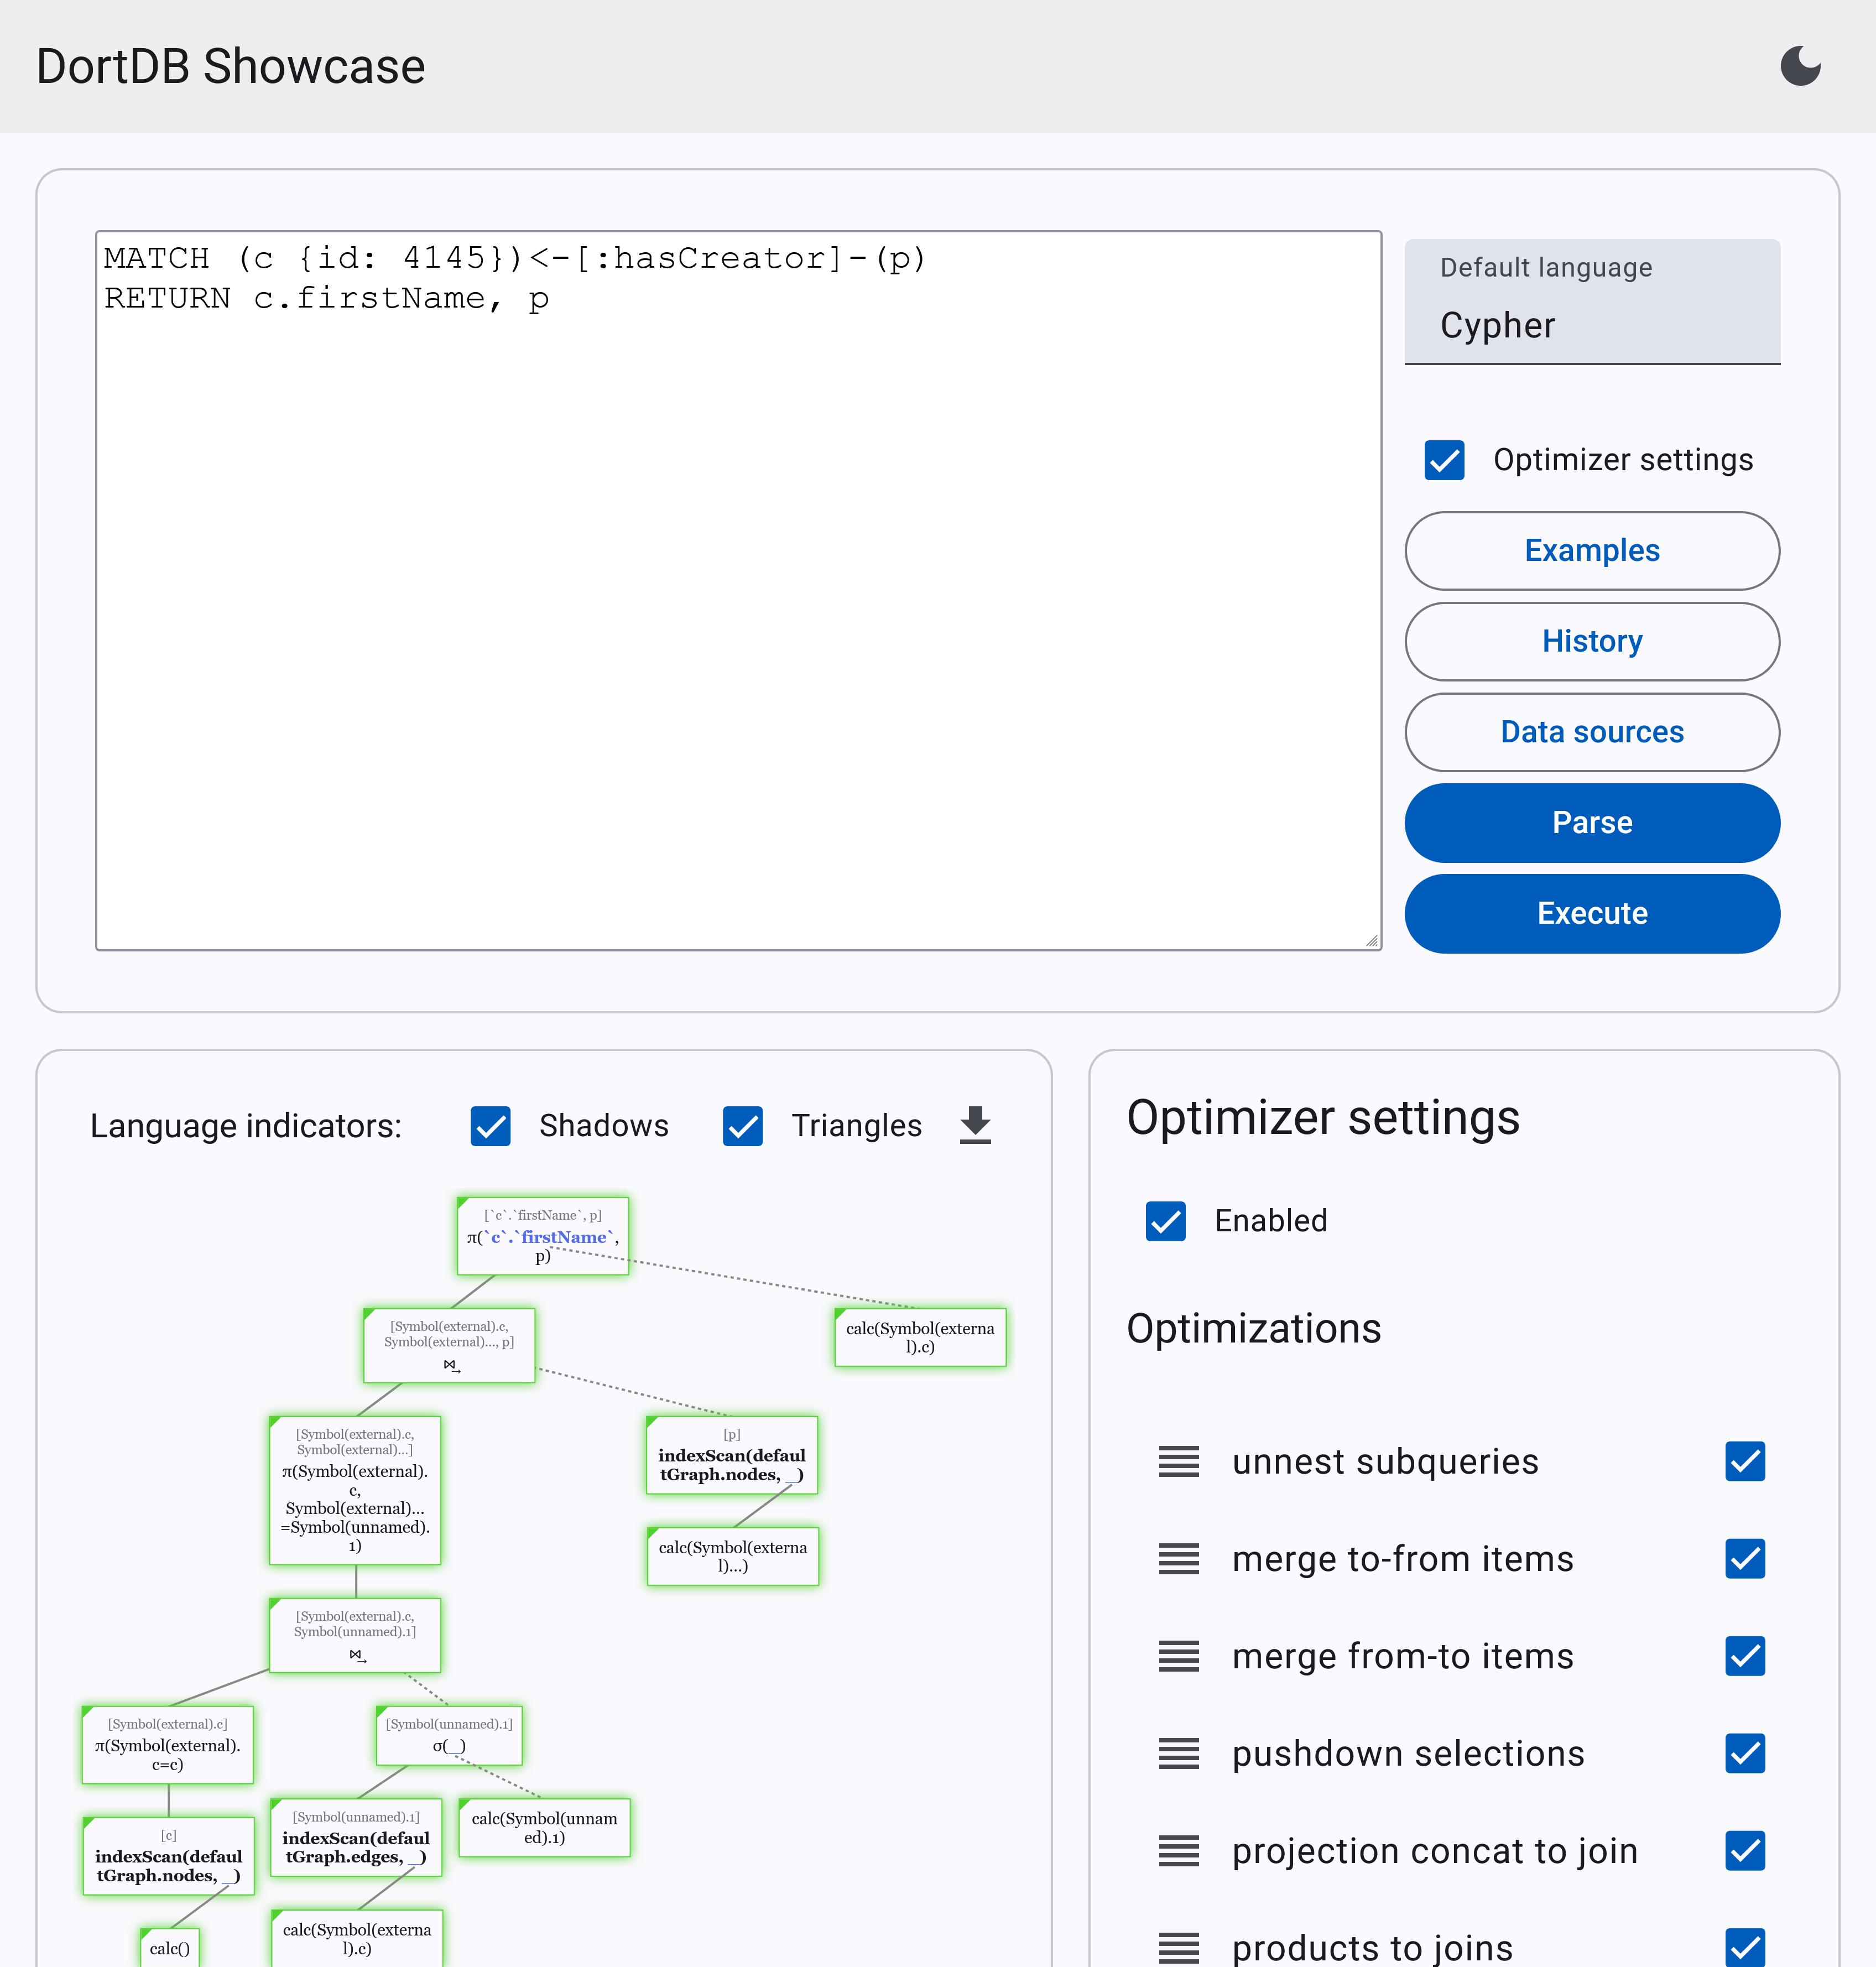
\includegraphics[width=0.8\linewidth]{img/showcase_optimizer.png}
    \caption{Showcase optimizer settings. The optimizer can be completely turned off. It is also possible to disable individual rules or to reorder them using drag \& drop.}
\end{figure}

\clearpage
\section{Programmatic usage}

The main class of the DortDB framework is simply called \texttt{DortDB}. It serves as the container for languages and extensions and exposes methods for registering data sources or querying. When creating a \texttt{DortDB} instance, it is necessary to provide at least one language. In order to facilitate better tree shaking, the optimizer, by default, receives no rules. However, all currently available rules are exported in a single array, already ordered for best performance. The individual languages can also be configured, for example, to use a different data adapter. The DortDB configuration can also specify additional user-defined functions, operators, or aggregates. It is also possible to bundle functions, operators, and aggregates into a single importable object called an extension. DortDB already comes with a \texttt{datetime} extension for manipulating dates and times. Extensions can be scoped to specific languages only. Only some languages support user-defined operators, for example, SQL.

\begin{listing}[!ht]
\begin{minted}{ts}
import { datetime, DortDB } from '@dortdb/core';
import { defaultRules } from '@dortdb/core/optimizer';
import { SQL } from '@dortdb/lang-sql';
import { DomDataAdapter, XQuery } from '@dortdb/lang-xquery';
import { Cypher } from '@dortdb/lang-cypher';

const db = new DortDB({
  mainLang: SQL(),
  additionalLangs: [
    XQuery({
      // in browser environment
      adapter: new DomDataAdapter(document)
    }),
    Cypher({ defaultGraph: 'defaultGraph' })
  ],
  optimizer: {
    rules: defaultRules,
  },
  extensions: [
    datetime,
    {
      scope: ['cypher'],
      aggregates: [
        // ... aggregates only for Cypher
      ],
    },
  ],
});
\end{minted}
\caption{DortDB data sources registration.}
\end{listing}

Once a \texttt{DortDB} instance is created, data sources can be registered. All the registration does is a pairing of a data structure with an identifier. It is then possible to index the structure with secondary indices. The developer needs to specify which type of index is used.

\begin{listing}[!ht]
\begin{minted}[fontsize=\small]{ts}
import { MapIndex } from '@dortdb/core';
import { MultiDirectedGraph } from 'graphology';

// db is already initialized
const arr = [1, 2, 3];
const obj = { prop: 'value' };
const objArr = [obj];

// the identifiers can have multiple parts
db.registerSource(['testing', 'arr'], arr);
db.registerSource(['testing', 'objArr'], objArr);
// anything can be registered, it is up to 
// the language data adapters to use it
db.registerSource(['testing', 'obj'], obj);
db.registerSource(['defaultGraph'], new MultiDirectedGraph());

// a simple hash index
// some indices may support indexing multiple expressions
db.createIndex(['testing', 'objArr'], ['prop'], MapIndex);
// the indexed expression is parsed with the default language
// but this can be changed by passing in a config parameter
db.createIndex(['testing', 'objArr'], ['prop->2'], MapIndex);

// for data sources that should be interpreted as item sources
// a specific identifier is configured to be treated as the item
// while parsing the expression
db.createIndex(['defaultGraph', 'nodes'], ['x.id'], MapIndex, {
  mainLang: 'cypher',
  fromItemKey: ['x'],
});
\end{minted}
\caption{DortDB initial setup.}
\end{listing}

\begin{listing}[!ht]
\begin{minted}[fontsize=\small]{ts}
import { UnnestSubqueries } from '@dortdb/core/optimizer';

db.optimizer.reconfigure({
  rules: [UnnestSubqueries]
});
\end{minted}
\caption{The query optimizer can be reconfigured at any time.}
\end{listing}

After the database is fully configured, we can parse queries into an AST, build and optimize logical plans, and execute them. Both the AST and the logical plan implement the visitor design pattern, so additional preprocessing can be added. All of the logical plan operators also expose a \texttt{getChildren()} method, so it is possible to quickly and simply iterate through the whole operator tree.

\begin{listing}[!ht]
\begin{minted}[fontsize=\small]{ts}
import { ASTNode } from '@dortdb/core';
import * as plan from '@dortdb/core/plan';

const query = 'SELECT a FROM t';

// some languages allow multiple statements
// per one query, so the result is an array
const ast: ASTNode[] = db.parse(query);

const plan = db.buildPlan(ast.at(-1));

// if we wanted to invert `orderBy` directions, we
// could write a visitor, or do it the quick way:
const stack = [plan];
while (stack.length) {
  const current = stack.pop();
  stack.push(...current.getChildren());
  if (current instanceof plan.Order) {
    for (const o of current.orders) {
      o.ascending = !o.ascending;
    }
  }
}

const results = db.executePlan(plan);

// during the relevant phases, the default language
// can be changed, and bound parameters can be provided

// we can also just query without caring about the plan or AST
const newResults = db.query(`
  MATCH (a)-[]->(b)
  WHERE a.id > $id
  RETURN a, b
`, {
  mainLang: 'cypher',
  boundParams: { id: 13 }
});
\end{minted}
\caption{Querying the database.}
\end{listing}

\section{Extensibility}
\label{sec:usage-extensibility}

One of DortDB's main selling points is its extensibility. It is possible (and encouraged) to provide more languages, index types, optimizer rules, or extensions. This section aims to outline in broad steps how to do all of the above-mentioned.

\subsection{Authoring a new language}

First of all, it is necessary to implement a parser that will parse the language queries into an AST. The parser must recognize language switches and switch to a different parser and then resume parsing afterward. To this end, each parser must recognize when to end even if there is yet remaining input, be it because of an encountered \texttt{LANG EXIT} token or because the parser would exit its initial scope. The parser should return both the parsed AST and any remaining unparsed input, so that an outer parser could continue, as in Program \ref{fig:parser-exit}.

\begin{listing}[!ht]
\begin{minted}{sql}
SELECT t1.attr1 FROM (
  LANG newlang
  -- new language here...
) AS t1 WHERE attr1 > 3
\end{minted}
\caption{The nested language should recognize the closing parenthesis as a scope exit and terminate. It should return both the parsed AST and the remaining input string \mintinline{sql}{) AS t1 WHERE attr1 > 3}.}
\label{fig:parser-exit}
\end{listing}

After the AST is available, the language should build an initial logical plan. If the unified algebra does not suffice, the language can define its own plan operators. It must, however, extend all core visitors to take these new operators into account. When building the plan, the language will receive an \texttt{IdSet} with identifiers defined in the outer context. Some of the identifiers in the \texttt{IdSet} may have the \texttt{Symbol(toInfer)} as their last token. This means that the identifier belongs to a data source whose schema is still being inferred. If the language encounters any matching identifiers, it should record them and return them in addition to the built logical plan.

\begin{listing}[!ht]
\begin{minted}[fontsize=\small]{ts}
import { AttributeRenamer, PlanVisitor } from '@dortdb/core';
import { TreeJoin, XQueryPlanVisitor } from '../plan/index.js';
import { RenameMap } from '@dortdb/core/plan';

export class XQueryAttributeRenamer
  extends AttributeRenamer
  implements XQueryPlanVisitor<void, RenameMap>
{
  // ...
  visitTreeJoin(operator: TreeJoin, renames: RenameMap): void {
    operator.source.accept(this.vmap, renames);
    this.processItem(operator, 'step', operator.dependencies, renames);
  }
}

// in language.ts:

export function XQuery(config?: XQueryConfig): XQueryLanguage {
  return {
    name: 'xquery',
    // ...
    visitors: {
      attributeRenamer: XQueryAttributeRenamer,
      // ...
    },
  };
}
\end{minted}
\caption{When extending the unified algebra, all core visitors must be extended as well. This example is taken from \texttt{@dortdb/lang-xquery}.}
\end{listing}

\subsection{Authoring a new index type}

DortDB features secondary indices. The index must implement the following three methods: \texttt{match}, to receive an array of expressions and decide whether some match the index. \texttt{CreateAccessor}, which takes an array of expressions that match the index, and should return a \texttt{calculation} which accesses the index and finds matching items for specific values of the expressions. Finally, there is the \texttt{reindex} method, which receives items from the connected data source and values of the indexed expressions, and should fill the index data structure.

The index does not always need to store the data in any structure. For example, the Cypher \texttt{ConnectionIndex} detects join conditions between nodes and edges, and then selects connected edges or nodes using the Cypher data adapter.

\subsection{Authoring other components}

Besides entire languages or specialized secondary indices, DortDB can also be extended with new optimizer rules. This may be especially relevant for custom logical plan operators. The rules may be as simple as removing neighboring \texttt{mapFromItem} and \texttt{mapToItem}, or complex algorithms for merging \texttt{Projections}. In all cases, they can be reduced to two methods: \texttt{match}, which recognizes patterns in the logical plan, and \texttt{transform}, which replaces the patterns with other patterns.

Finally, DortDB users may define their own functions or aggregates. These may be grouped into and distributed as extensions, for example, for spatial data manipulation or for the creation of dynamic data sources.